% Options for packages loaded elsewhere
\PassOptionsToPackage{unicode}{hyperref}
\PassOptionsToPackage{hyphens}{url}
\PassOptionsToPackage{dvipsnames,svgnames,x11names}{xcolor}
%
\documentclass[
  10pt,
  ignorenonframetext,
]{beamer}
\usepackage{pgfpages}
\setbeamertemplate{caption}[numbered]
\setbeamertemplate{caption label separator}{: }
\setbeamercolor{caption name}{fg=normal text.fg}
\beamertemplatenavigationsymbolsempty
% Prevent slide breaks in the middle of a paragraph
\widowpenalties 1 10000
\raggedbottom
\setbeamertemplate{part page}{
  \centering
  \begin{beamercolorbox}[sep=16pt,center]{part title}
    \usebeamerfont{part title}\insertpart\par
  \end{beamercolorbox}
}
\setbeamertemplate{section page}{
  \centering
  \begin{beamercolorbox}[sep=12pt,center]{part title}
    \usebeamerfont{section title}\insertsection\par
  \end{beamercolorbox}
}
\setbeamertemplate{subsection page}{
  \centering
  \begin{beamercolorbox}[sep=8pt,center]{part title}
    \usebeamerfont{subsection title}\insertsubsection\par
  \end{beamercolorbox}
}
\AtBeginPart{
  \frame{\partpage}
}
\AtBeginSection{
  \ifbibliography
  \else
    \frame{\sectionpage}
  \fi
}
\AtBeginSubsection{
  \frame{\subsectionpage}
}
\usepackage{amsmath,amssymb}
\usepackage{iftex}
\ifPDFTeX
  \usepackage[T1]{fontenc}
  \usepackage[utf8]{inputenc}
  \usepackage{textcomp} % provide euro and other symbols
\else % if luatex or xetex
  \usepackage{unicode-math} % this also loads fontspec
  \defaultfontfeatures{Scale=MatchLowercase}
  \defaultfontfeatures[\rmfamily]{Ligatures=TeX,Scale=1}
\fi
\usepackage{lmodern}
\usetheme[]{Singapore}
\usefonttheme{serif}
\ifPDFTeX\else
  % xetex/luatex font selection
\fi
% Use upquote if available, for straight quotes in verbatim environments
\IfFileExists{upquote.sty}{\usepackage{upquote}}{}
\IfFileExists{microtype.sty}{% use microtype if available
  \usepackage[]{microtype}
  \UseMicrotypeSet[protrusion]{basicmath} % disable protrusion for tt fonts
}{}
\makeatletter
\@ifundefined{KOMAClassName}{% if non-KOMA class
  \IfFileExists{parskip.sty}{%
    \usepackage{parskip}
  }{% else
    \setlength{\parindent}{0pt}
    \setlength{\parskip}{6pt plus 2pt minus 1pt}}
}{% if KOMA class
  \KOMAoptions{parskip=half}}
\makeatother
\usepackage{xcolor}
\newif\ifbibliography
\usepackage{color}
\usepackage{fancyvrb}
\newcommand{\VerbBar}{|}
\newcommand{\VERB}{\Verb[commandchars=\\\{\}]}
\DefineVerbatimEnvironment{Highlighting}{Verbatim}{commandchars=\\\{\}}
% Add ',fontsize=\small' for more characters per line
\usepackage{framed}
\definecolor{shadecolor}{RGB}{248,248,248}
\newenvironment{Shaded}{\begin{snugshade}}{\end{snugshade}}
\newcommand{\AlertTok}[1]{\textcolor[rgb]{0.94,0.16,0.16}{#1}}
\newcommand{\AnnotationTok}[1]{\textcolor[rgb]{0.56,0.35,0.01}{\textbf{\textit{#1}}}}
\newcommand{\AttributeTok}[1]{\textcolor[rgb]{0.13,0.29,0.53}{#1}}
\newcommand{\BaseNTok}[1]{\textcolor[rgb]{0.00,0.00,0.81}{#1}}
\newcommand{\BuiltInTok}[1]{#1}
\newcommand{\CharTok}[1]{\textcolor[rgb]{0.31,0.60,0.02}{#1}}
\newcommand{\CommentTok}[1]{\textcolor[rgb]{0.56,0.35,0.01}{\textit{#1}}}
\newcommand{\CommentVarTok}[1]{\textcolor[rgb]{0.56,0.35,0.01}{\textbf{\textit{#1}}}}
\newcommand{\ConstantTok}[1]{\textcolor[rgb]{0.56,0.35,0.01}{#1}}
\newcommand{\ControlFlowTok}[1]{\textcolor[rgb]{0.13,0.29,0.53}{\textbf{#1}}}
\newcommand{\DataTypeTok}[1]{\textcolor[rgb]{0.13,0.29,0.53}{#1}}
\newcommand{\DecValTok}[1]{\textcolor[rgb]{0.00,0.00,0.81}{#1}}
\newcommand{\DocumentationTok}[1]{\textcolor[rgb]{0.56,0.35,0.01}{\textbf{\textit{#1}}}}
\newcommand{\ErrorTok}[1]{\textcolor[rgb]{0.64,0.00,0.00}{\textbf{#1}}}
\newcommand{\ExtensionTok}[1]{#1}
\newcommand{\FloatTok}[1]{\textcolor[rgb]{0.00,0.00,0.81}{#1}}
\newcommand{\FunctionTok}[1]{\textcolor[rgb]{0.13,0.29,0.53}{\textbf{#1}}}
\newcommand{\ImportTok}[1]{#1}
\newcommand{\InformationTok}[1]{\textcolor[rgb]{0.56,0.35,0.01}{\textbf{\textit{#1}}}}
\newcommand{\KeywordTok}[1]{\textcolor[rgb]{0.13,0.29,0.53}{\textbf{#1}}}
\newcommand{\NormalTok}[1]{#1}
\newcommand{\OperatorTok}[1]{\textcolor[rgb]{0.81,0.36,0.00}{\textbf{#1}}}
\newcommand{\OtherTok}[1]{\textcolor[rgb]{0.56,0.35,0.01}{#1}}
\newcommand{\PreprocessorTok}[1]{\textcolor[rgb]{0.56,0.35,0.01}{\textit{#1}}}
\newcommand{\RegionMarkerTok}[1]{#1}
\newcommand{\SpecialCharTok}[1]{\textcolor[rgb]{0.81,0.36,0.00}{\textbf{#1}}}
\newcommand{\SpecialStringTok}[1]{\textcolor[rgb]{0.31,0.60,0.02}{#1}}
\newcommand{\StringTok}[1]{\textcolor[rgb]{0.31,0.60,0.02}{#1}}
\newcommand{\VariableTok}[1]{\textcolor[rgb]{0.00,0.00,0.00}{#1}}
\newcommand{\VerbatimStringTok}[1]{\textcolor[rgb]{0.31,0.60,0.02}{#1}}
\newcommand{\WarningTok}[1]{\textcolor[rgb]{0.56,0.35,0.01}{\textbf{\textit{#1}}}}
\usepackage{graphicx}
\makeatletter
\def\maxwidth{\ifdim\Gin@nat@width>\linewidth\linewidth\else\Gin@nat@width\fi}
\def\maxheight{\ifdim\Gin@nat@height>\textheight\textheight\else\Gin@nat@height\fi}
\makeatother
% Scale images if necessary, so that they will not overflow the page
% margins by default, and it is still possible to overwrite the defaults
% using explicit options in \includegraphics[width, height, ...]{}
\setkeys{Gin}{width=\maxwidth,height=\maxheight,keepaspectratio}
% Set default figure placement to htbp
\makeatletter
\def\fps@figure{htbp}
\makeatother
\setlength{\emergencystretch}{3em} % prevent overfull lines
\providecommand{\tightlist}{%
  \setlength{\itemsep}{0pt}\setlength{\parskip}{0pt}}
\setcounter{secnumdepth}{-\maxdimen} % remove section numbering
\usepackage{multirow}
\ifLuaTeX
  \usepackage{selnolig}  % disable illegal ligatures
\fi
\IfFileExists{bookmark.sty}{\usepackage{bookmark}}{\usepackage{hyperref}}
\IfFileExists{xurl.sty}{\usepackage{xurl}}{} % add URL line breaks if available
\urlstyle{same}
\hypersetup{
  pdftitle={Module 10: Unsupervised learning (Overview/quizz lecture)},
  pdfauthor={Sara Martino, Department of Mathematical Sciences, NTNU},
  colorlinks=true,
  linkcolor={Maroon},
  filecolor={Maroon},
  citecolor={Blue},
  urlcolor={blue},
  pdfcreator={LaTeX via pandoc}}

\title{Module 10: Unsupervised learning (Overview/quizz lecture)}
\subtitle{TMA4268 Statistical Learning V2023}
\author{Sara Martino, Department of Mathematical Sciences, NTNU}
\date{April 5, 2024}

\begin{document}
\frame{\titlepage}

\begin{frame}[fragile]
\begin{block}{PCA example}
\protect\hypertarget{pca-example}{}
\(~\)

\begin{itemize}
\item
  We study the \texttt{decathlon2} dataset from the \texttt{factoextra}
  package in R, where Athletes' performance during a sporting meeting
  was recorded.
\item
  We look at 23 athletes and the results from the 10 disciplines in two
  competitions.
\end{itemize}

\begin{Shaded}
\begin{Highlighting}[]
\FunctionTok{library}\NormalTok{(factoextra)}
\FunctionTok{library}\NormalTok{(FactoMineR)}
\FunctionTok{data}\NormalTok{(}\StringTok{"decathlon2"}\NormalTok{)}
\NormalTok{decathlon2.active }\OtherTok{\textless{}{-}}\NormalTok{ decathlon2[}\DecValTok{1}\SpecialCharTok{:}\DecValTok{23}\NormalTok{, }\DecValTok{1}\SpecialCharTok{:}\DecValTok{10}\NormalTok{]}
\FunctionTok{names}\NormalTok{(decathlon2.active) }\OtherTok{\textless{}{-}} \FunctionTok{c}\NormalTok{(}\StringTok{"100m"}\NormalTok{, }\StringTok{"long\_jump"}\NormalTok{, }\StringTok{"shot\_put"}\NormalTok{, }\StringTok{"high\_jump"}\NormalTok{,}
    \StringTok{"400m"}\NormalTok{, }\StringTok{"110.hurdle"}\NormalTok{, }\StringTok{"discus"}\NormalTok{, }\StringTok{"pole\_vault"}\NormalTok{, }\StringTok{"javeline"}\NormalTok{, }\StringTok{"1500m"}\NormalTok{)}
\end{Highlighting}
\end{Shaded}

\(~\)

\scriptsize

\begin{verbatim}
##          100m long_jump shot_put high_jump  400m 110.hurdle discus pole_vault
## SEBRLE  11.04      7.58    14.83      2.07 49.81      14.69  43.75       5.02
## BERNARD 11.02      7.23    14.25      1.92 48.93      14.99  40.87       5.32
## YURKOV  11.34      7.09    15.19      2.10 50.42      15.31  46.26       4.72
##         javeline 1500m
## SEBRLE     63.19 291.7
## BERNARD    62.77 280.1
## YURKOV     63.44 276.4
\end{verbatim}
\end{block}
\end{frame}

\begin{frame}
\begin{figure}
\includegraphics[width=0.55\linewidth]{10Unsuper_files/figure-beamer/biplot-1} \end{figure}
\end{frame}

\begin{frame}
\begin{block}{Proportion of varianced explained (PVE)}
\protect\hypertarget{proportion-of-varianced-explained-pve}{}
\(~\)

\textbf{Recap:} The PVE by PC \(m\) is given by

\[
\frac{\sum_{i=1}^m z_{im}^2} {\sum_{j=1}^p\sum_{i=1}^n x_{ij}^2}
\]
\end{block}
\end{frame}

\begin{frame}
\begin{block}{Scree plot}
\protect\hypertarget{scree-plot}{}
\(~\)

A graphical description of the \textbf{proportion of variance explained
(PVE)} by a certain number of PCs:

\centering

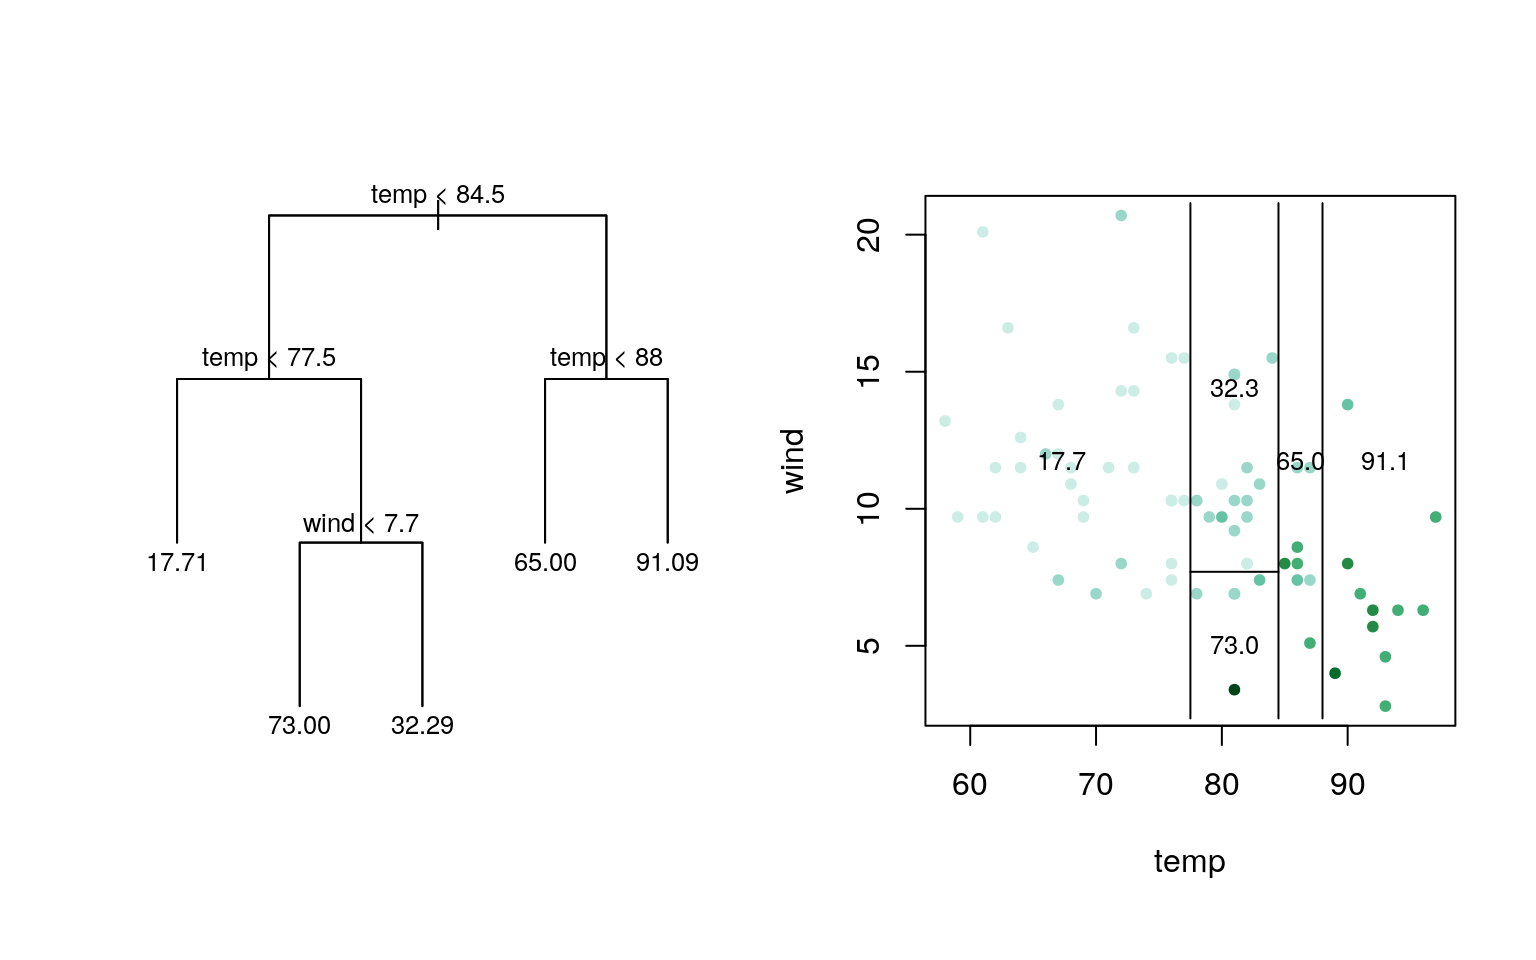
\includegraphics[width=0.9\linewidth]{10Unsuper_files/figure-beamer/unnamed-chunk-5-1}
\end{block}
\end{frame}

\begin{frame}[fragile]{Another example}
\protect\hypertarget{another-example}{}
Protein consumption in twenty-five European countries for nine food
groups.

\begin{verbatim}
##                Red_Meat White_Meat Eggs Milk Fish Cereal Starch Nuts
## Albania            10.1        1.4  0.5  8.9  0.2   42.3    0.6  5.5
## Austria             8.9       14.0  4.3 19.9  2.1   28.0    3.6  1.3
## Belgium            13.5        9.3  4.1 17.5  4.5   26.6    5.7  2.1
## Bulgaria            7.8        6.0  1.6  8.3  1.2   56.7    1.1  3.7
## Czechoslovakia      9.7       11.4  2.8 12.5  2.0   34.3    5.0  1.1
## Denmark            10.6       10.8  3.7 25.0  9.9   21.9    4.8  0.7
##                Fruits_Vegetables
## Albania                      1.7
## Austria                      4.3
## Belgium                      4.0
## Bulgaria                     4.2
## Czechoslovakia               4.0
## Denmark                      2.4
\end{verbatim}
\end{frame}

\begin{frame}{Correlation Matrix}
\protect\hypertarget{correlation-matrix}{}
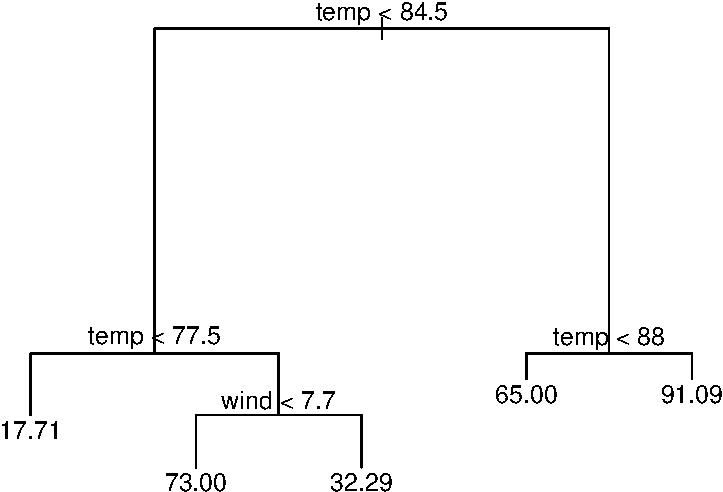
\includegraphics{10Unsuper_files/figure-beamer/unnamed-chunk-7-1.pdf}
\end{frame}

\begin{frame}{PCA}
\protect\hypertarget{pca}{}
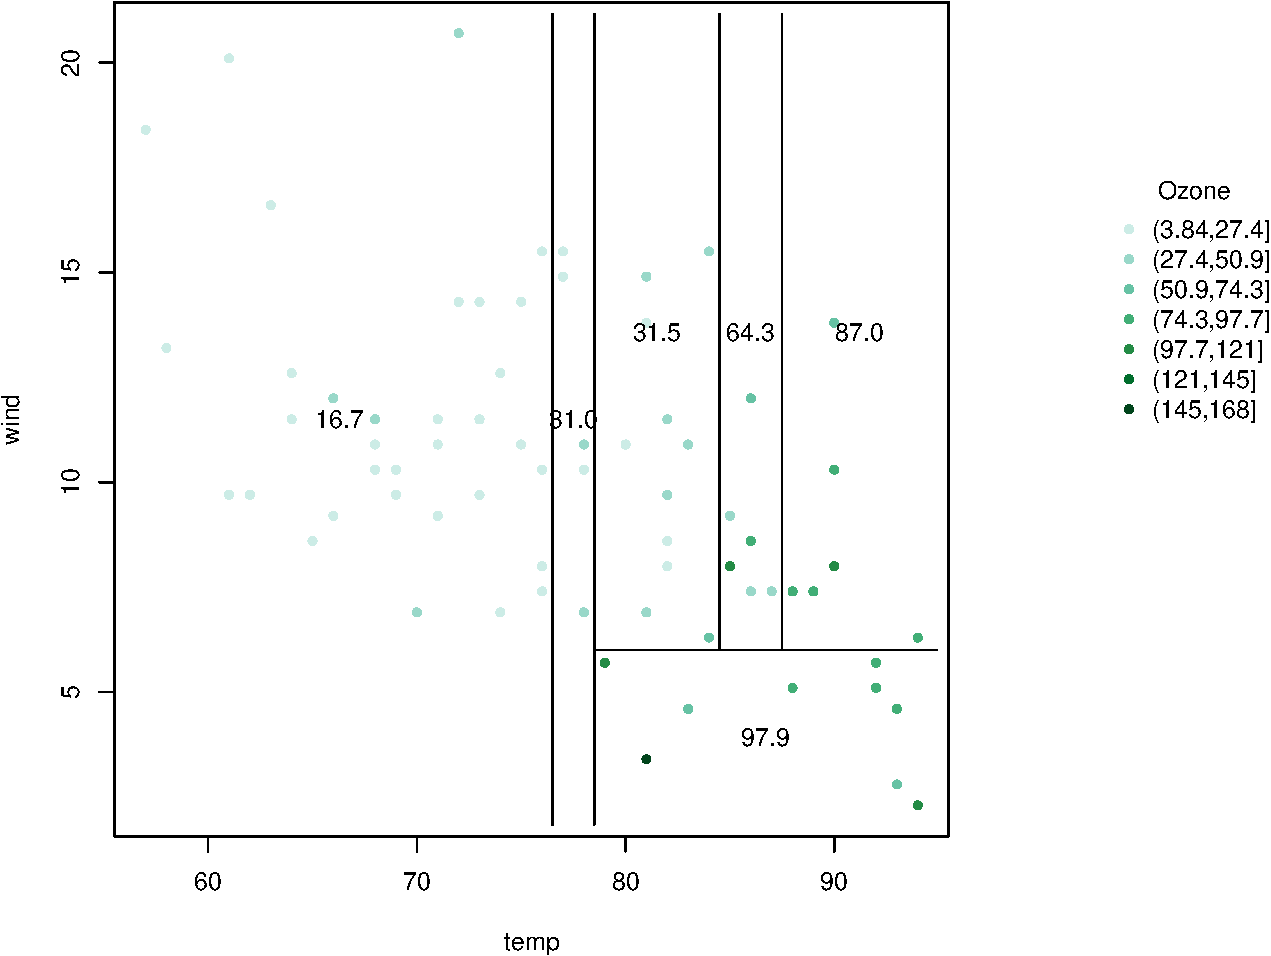
\includegraphics{10Unsuper_files/figure-beamer/unnamed-chunk-8-1.pdf}
\end{frame}

\begin{frame}[fragile]{Variance Explained}
\protect\hypertarget{variance-explained}{}
\footnotesize

\begin{verbatim}
## Importance of components:
##                           PC1    PC2    PC3    PC4     PC5     PC6     PC7
## Standard deviation     2.0016 1.2787 1.0620 0.9771 0.68106 0.57020 0.52116
## Proportion of Variance 0.4452 0.1817 0.1253 0.1061 0.05154 0.03613 0.03018
## Cumulative Proportion  0.4452 0.6268 0.7521 0.8582 0.90976 0.94589 0.97607
##                            PC8     PC9
## Standard deviation     0.34102 0.31482
## Proportion of Variance 0.01292 0.01101
## Cumulative Proportion  0.98899 1.00000
\end{verbatim}
\end{frame}

\begin{frame}{Variance Explained - Scree plot}
\protect\hypertarget{variance-explained---scree-plot}{}
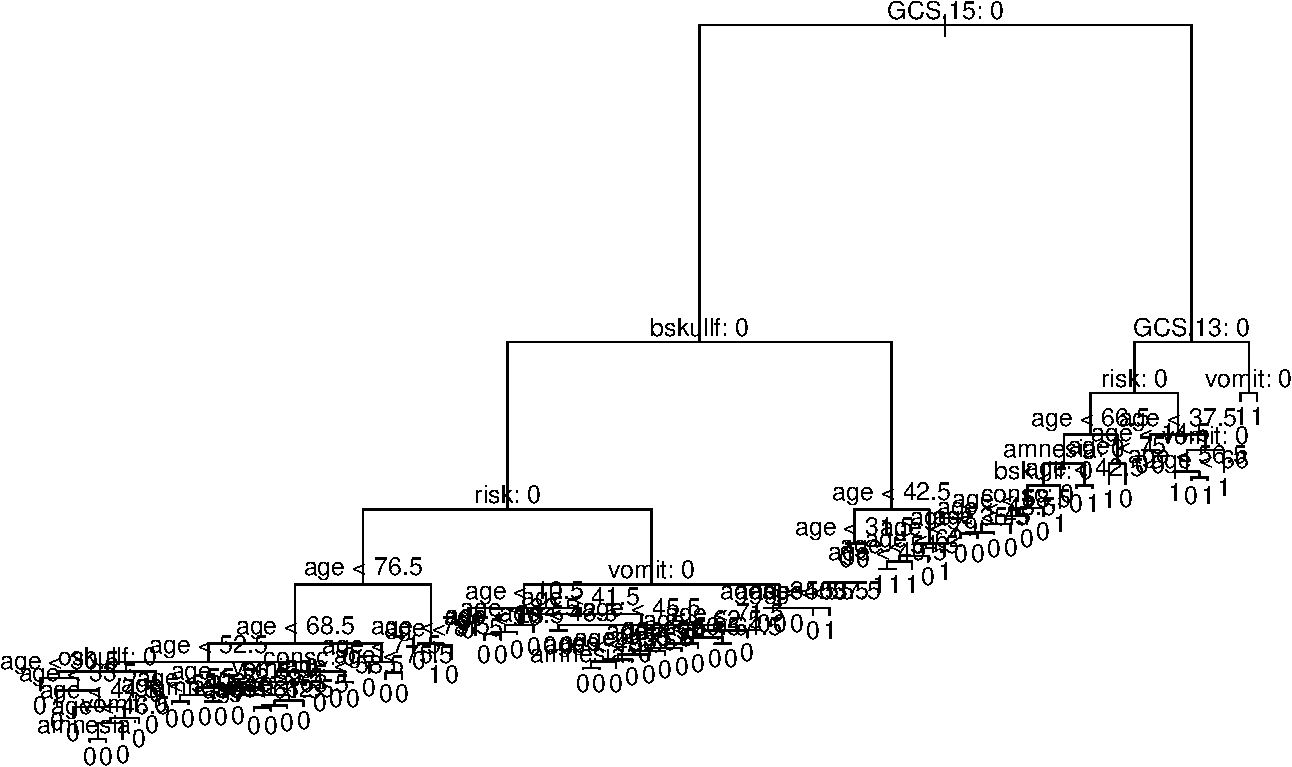
\includegraphics{10Unsuper_files/figure-beamer/unnamed-chunk-10-1.pdf}
\end{frame}

\begin{frame}{Clustering}
\protect\hypertarget{clustering}{}
\(~\)

\begin{itemize}
\item
  The aim is to find \emph{clusters} or \emph{subgroups}.
\item
  Clustering looks for homogeneous subgroups in the data.
\end{itemize}

\(~\)

Difference to PCA?

\pause

\(\rightarrow\) PCA looks for low-dimensional representation of the
data.
\end{frame}

\begin{frame}
\begin{block}{K-means vs.~hierarchical clustering}
\protect\hypertarget{k-means-vs.-hierarchical-clustering}{}
\(~\)

See menti.com
\end{block}
\end{frame}

\begin{frame}
\begin{block}{K-means clustering}
\protect\hypertarget{k-means-clustering}{}
\(~\)

\begin{itemize}
\tightlist
\item
  Fix the number of clusters \(K\).
\end{itemize}

\(~\)

\begin{itemize}
\tightlist
\item
  Find groups such that the sum of the within-cluster variation is
  minimized.
\end{itemize}

\(~\)
\end{block}
\end{frame}

\begin{frame}{K-means clustering - Algorithm}
\protect\hypertarget{k-means-clustering---algorithm}{}
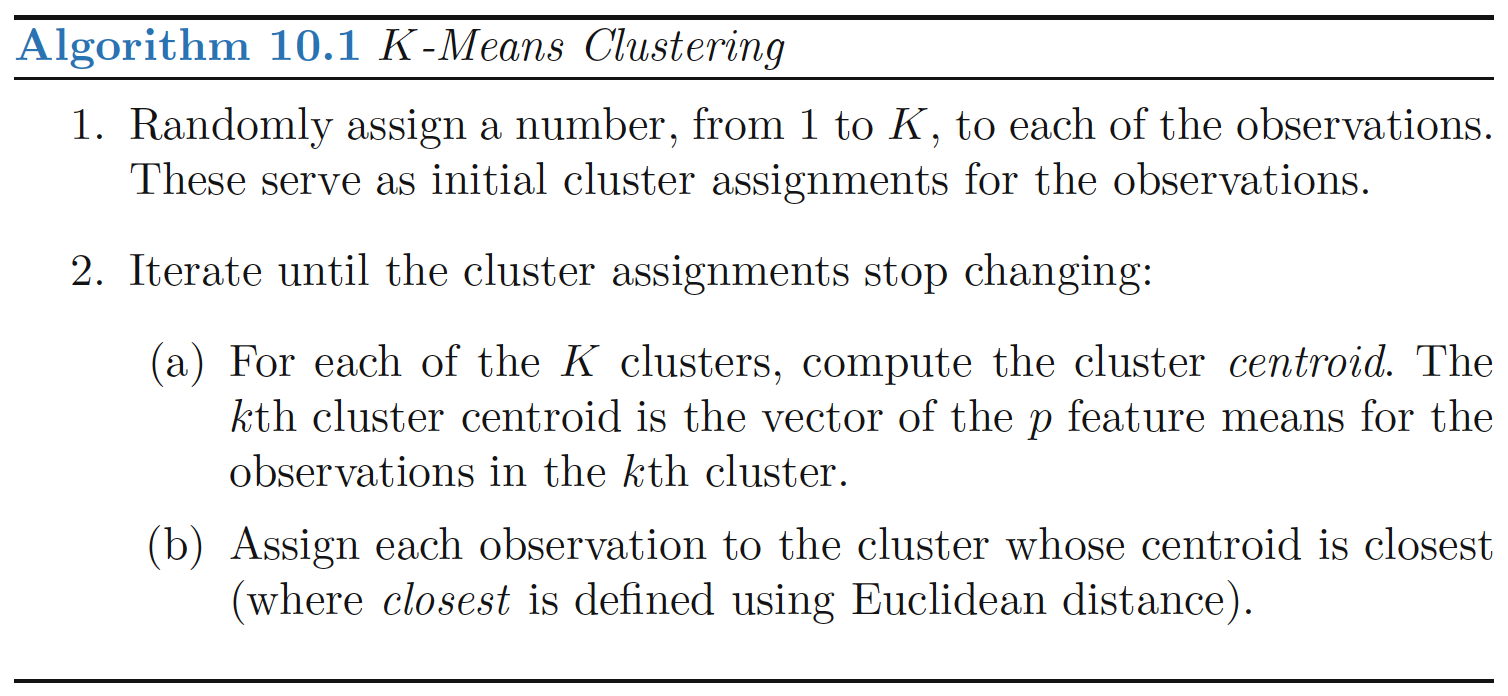
\includegraphics{imgs/kmeans_algo.png}
\end{frame}

\begin{frame}
\begin{block}{Hierarchical clustering}
\protect\hypertarget{hierarchical-clustering}{}
\(~\)

Bottom-up agglomerative clustering that results in a
\emph{\textcolor{red}{dendogram}}.

\(~\)

\includegraphics{imgs/hierarchical_algorithm.png}
\end{block}
\end{frame}

\begin{frame}
\begin{block}{Important in hierarchical clustering}
\protect\hypertarget{important-in-hierarchical-clustering}{}
\(~\)

\begin{itemize}
\tightlist
\item
  \emph{\textcolor{red}{Linkage:}} Complete, single, average centroid.
\end{itemize}

\(~\)

\begin{itemize}
\tightlist
\item
  \emph{\textcolor{red}{Dissimilarity measure:}} Euclidian distance,
  correlation. \emph{Other similarity/distance measures?}
  \footnote{ Note: Correlation is actually a similarity measure, not a distance measure. Implication?}
\end{itemize}
\end{block}
\end{frame}

\begin{frame}
\begin{block}{Hierarchical clustering -- example}
\protect\hypertarget{hierarchical-clustering-example}{}
\(~\)

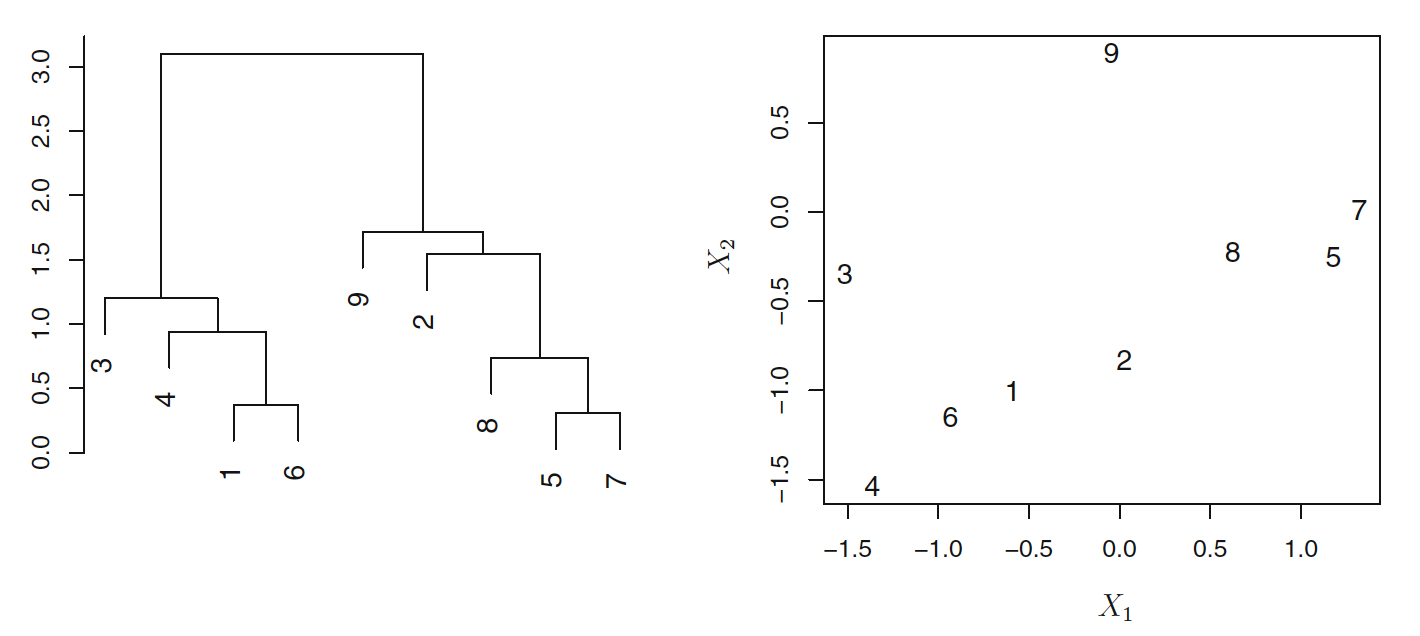
\includegraphics{imgs/dendogram_misleading.png}

Note: The representation on the right is not possible in
high-dimensional space (i.e., if we have \(X_1, X_2, X_3, ...., X_p\)).
\end{block}
\end{frame}

\begin{frame}{Exercise 2 from the book}
\protect\hypertarget{exercise-2-from-the-book}{}
We have the following dissimilarity matrix:

\[\begin{bmatrix}0&0.3&0.4&0.7 \\0.3&0&0.5&0.8 \\0.4&0.5&0&0.45 \\0.7&0.8&0.45&0 \\\end{bmatrix}\]

\begin{enumerate}
\item
  Sketch the dendogram using \emph{complete} linkage, indicate on the
  plot the height at wich each fusion occurs, as well as the
  observations corresponding to each leaf in the dendogram
\item
  Repeat using \emph{single} linkage
\item
  Suppose we cut the two dendograms such that 2 clusters result. Which
  observations are in each cluster?
\end{enumerate}
\end{frame}

\begin{frame}{Exercise 11 from the book}
\protect\hypertarget{exercise-11-from-the-book}{}
\includegraphics{imgs/Ch10_ex11.png}
\end{frame}

\begin{frame}
\begin{block}{Pros and cons of clusterization methods / practical
issues}
\protect\hypertarget{pros-and-cons-of-clusterization-methods-practical-issues}{}
\(~\)

\(~\)

\(~\)

\(~\)

\(~\)

\(~\)

\(~\)

\(~\)

\(~\)

\(~\)
\end{block}
\end{frame}

\begin{frame}{References}
\protect\hypertarget{references}{}
\end{frame}

\end{document}
